% ==============================================================================
% Tese - Marcos Alécio Spalenza
% Capítulo 2 - Revisão da Literatura
% ==============================================================================
\chapter{Revisão da Literatura}
\label{cap-literatura}

A sala de aula é um ambiente que produz diariamente grande quantidade de informações. As informações são essenciais para o acompanhar do aprendizado dos alunos, verificar a necessidade de reforço do conteúdo e monitorar o cumprimento do curricular. Tradicionalmente essa dinâmica faz parte dos métodos de ensino-aprendizagem empregados pelos professores, porém, superam a capacidade analítica dos mesmos \cite{madero2019}. Por conta disso, para ampliar a verificação do professor em analisar os materiais produzidos em sala, ganharam maior notoriedade e espaço prático os sistemas de EDM \cite{siemens2012, romero2010}.

Em EDM, métodos de extração de informação são aplicados aos dados da classe de alunos para a aquisição de conhecimento, apoio ao tutor e acompanhamento do ensino \cite{ferreiramello2019}. Através de técnicas de ML, ocorre a redução da carga do professor para tratamento e acompanhamento do conteúdo ministrado em sala. Deste modo, o professor torna-se responsável pela auditoria, monitoramento e aplicação dos resultados obtidos. Assim, os sistemas apoiam a descoberta de problemas de aprendizado, a personalização do ensino e a acompanhamento coletivo dos alunos em sala. 

Portanto, através da mineração de dados, é possível ao professor a análise de todo material produzido pelos alunos, a criação de feedbacks individuais e a aplicação de reforço para determinados grupos de estudantes. Neste ponto, dentro dos métodos de EDM, um nicho de sistemas que tange diretamente essa demanda são os sistemas SAG \cite{burrows2015}. Os SAG são responsáveis pela verificação em massa das respostas textuais curtas, auxiliando o professor no processo de correção. É característico deste tipo de questão a verificação do aprendizado do aluno segundo o material ministrado em sala \cite{oliveira2013}. Ao aluno, este tipo de questão é fundamental para prática da escrita, busca de informações e sumarização do conteúdo em poucas palavras. Portanto, este tipo de atividade envolve métodos relevantes para todos os níveis de ensino, principalmente durante o aprendizado e desenvolvimento da escrita \cite{johnstone2002}.

Apesar da relevância das questões discursivas curtas, sua aplicação é gradativamente reduzida pela alta carga-horária do professor em sala \cite{bilgin2017}. Assim, torna-se uma demanda secundária o planejamento, a revisão e a análise do material dos alunos. O apoio computacional, reduz o tempo necessário fora da sala para avaliação do conteúdo, com o professor participando parcialmente do processo de avaliação \cite{ming2005}. O nicho dos métodos computacionais de apoio aos métodos avaliativos são conhecidos também por CAA \cite{perez-marin2009}. Neste processo, os resultados obtidos são auditados pelo professor para garantir que o modelo avaliativo foi seguido fielmente para que a representação do conhecimento das respostas atenda coerentemente as demandas da atividade. Enquanto isso, a aplicação de técnicas de ML reflete que a descrição do modelo de correção utilizado é um potencial \textit{feedback} com aplicação direta em sala \cite{butcher2010}.

Para o uso dos métodos de SAG, é importante que a questão seja elaborada com o objetivo de analisar os conhecimentos dos estudantes segundo um domínio específico \cite{bailey2008}. Comumente separamos as questões em discursivas e objetivas, de acordo com o modelo de resposta esperada. As questões discursivas \cite{bezerra2008} envolvem a liberdade de escrita do aluno, avaliando sua capacidade de descrição e desenvolvimento textual. Por outro lado as questões objetivas desenvolvem o raciocínio, a leitura e interpretação do material didático e a busca de informações. Sabendo disso, as questões discursivas permeiam ambos os tipos de habilidades do aluno. A Figura \ref{fig-atividades} caracteriza as atividades segundo os modelos de resposta \cite{burrows2015}.

\begin{figure}[h]
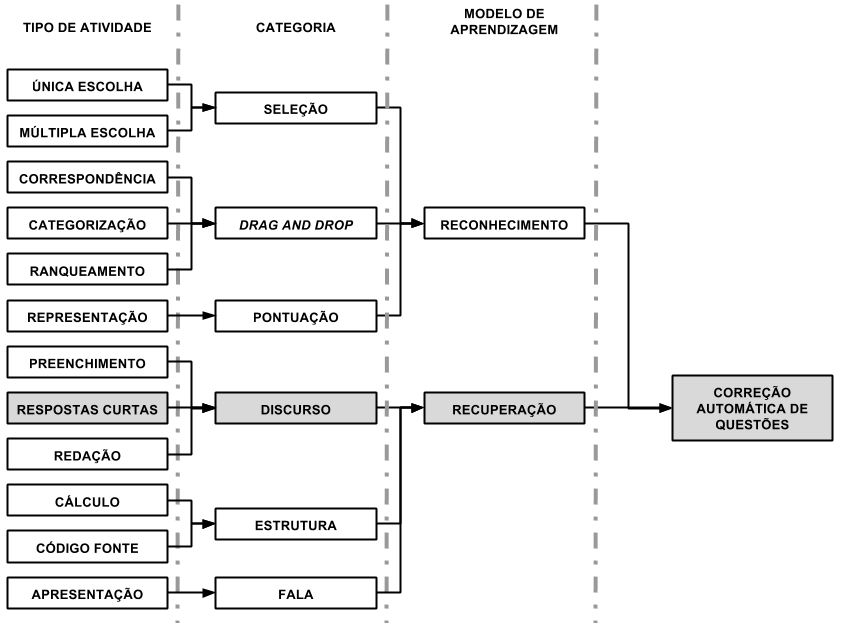
\includegraphics[width=\textwidth]{figuras/tiposAtividade}
\caption{A extração da informação e os tipos tradicionais de atividade aplicadas no cotidiano de sala de aula.}
\label{fig-atividades}
\end{figure}


Como apresentado na Figura \ref{fig-atividades} o professor dispõe de alguns modelos de atividades que, refletem diferentes aspectos do aprendizado. Dentre as redações de cunho aberto e irrestrito e as respostas diretas com opções elencadas no enunciado, as respostas discursivas encontram-se em âmbito intermediário \cite{bailey2008}. As respostas curtas buscam que o aluno estabeleça relação entre o aprendizado com material didático e a sua descrição textual. Assim, dentre os conhecimentos gerais, a questão deve evitar abordar temas de cunho interpretativo e que tangenciam experiências específicas de cada aluno \cite{siddiqi2008}. Por outro lado, a resposta deve representar a informação completa da questão, dando ao sistema embasamento para correção, evitando informações restritas ou codificadas \cite{ding2020}. A Figura \ref{fig-SAG-concepts} demonstra como o espectro de questões trabalhados através das respostas discursivas curtas.


\begin{figure}[h]
\begin{center}
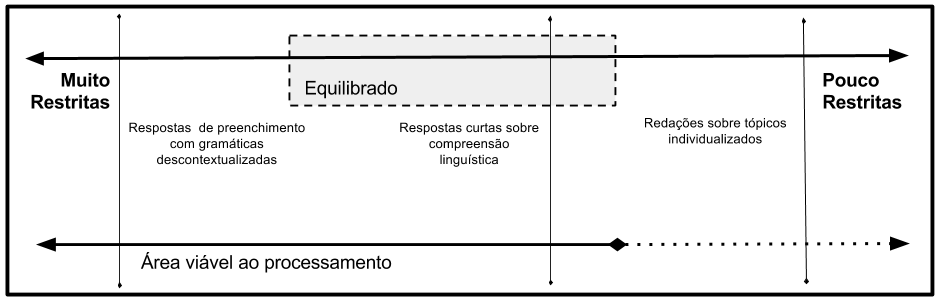
\includegraphics[width=\textwidth]{figuras/aprendizadoSAG}
\caption{Extração de informação em questões discursivas: entre respostas pequenas não-convergentes e a subjetividade das competências na avaliação de redações.}
\label{fig-SAG-concepts}
\end{center}
\end{figure}


A Figura \ref{fig-SAG-concepts} caracteriza exatamente, dentro do nicho de questões discursivas, a dinâmica de uso do processamento computacional das respostas por parte do professor. O ideal é que a questão direcione o aluno a uma ou poucas respostas, evitando várias respostas corretas divergentes \cite{suzen2020} ou questões longas e subjetivas como redações \cite{almeida-junior2017}. Quando as respostas não são únicas e apresentam um conhecimento comum não abstrato, é o ideal para uso dos métodos de correção automática. Portanto, é fundamental a convergência das respostas, para que as respostas apresentem uma ou poucas direções a serem abordadas pelos estudantes \cite{filighera2020}. Para isso, é fundamental que o sistema realize três passos. O primeiro é o aprendizado do modelo de respostas do aluno \cite{ramachandran2015b}. O segundo é através do modelo de respostas reconhecer o padrão avaliativo do professor \cite{funayama2020}. Por fim, no terceiro passo, o sistema deve replicar o modelo avaliativo e elaborar \textit{feedbacks} coerentes \cite{fowler2021}.

\section{Avaliação Semi-Supervisionada}

O método de aprendizado é o procedimento que dita a forma de aquisição de informações do sistema para criação de modelos com desempenho similar ao humano. Neste trabalho apresentamos um método de amostragem semi-supervisionado de aprendizado através da anotação do professor em itens selecionados através da \textit{clusterização} \cite{horbach2018}. Porém, a requisição de anotação do professor para amostras de respostas não é o método tradicional para modelo avaliativo.

A grande maioria dos trabalhos utiliza amostragem através do particionamento entre treino e teste dos dados, previamente selecionado nos \textit{datasets}. Considerando cada resposta dos estudantes uma amostra, o particionamento em treino e teste reflete a divisão \textit{a priori} do conjunto de dados em um grupo para criação do modelo e outro para avaliação \cite{heilman2015}. Esse modelo clássico permite ao sistema observar apenas uma parcela dos dados, onde o sistema realiza a inferência nos demais dados desconhecidos. Assim, o sistema deve absorver o modelo avaliativo do conjunto de treino e replicar o método avaliativo no conjunto de teste, pressupondo a equivalência dos mesmos. Porém, o modelo não necessariamente é similar ao de teste, não refletindo diretamente a aplicação de um sistema SAG em conjunto com o professor \cite{sung2019a}.

Outros métodos, mais próximos da demanda do professor, utilizam de exemplos anotados de respostas para criação de modelo \cite{banjade2015, roy2016}. Tais exemplos são denominadas respostas candidatas. As respostas candidatas, são amostras elaboradas pelo professor e anotadas para representar seus padrões avaliativos. Os sistemas SAG com base nesse tipo de dado buscam, em geral, a comparação direta entre as respostas e o índice de sobreposição \cite{kar2017, jimenez2013}. Porém, este tipo de treinamento gera uma tendência na avaliação, com limitada interpretação das respostas dos alunos \cite{ramachandran2015a}. O modelo criado não é capaz de identificar múltiplos contextos e as referências apresentadas pelo aluno. Portanto, as limitações da informação passada são um contraponto à liberdade textual esperada das atividades de escrita livre \cite{burrows2015}. Além de tornar-se engessada, não necessariamente são similares aos demais documentos do \textit{dataset}.

Para contornar as limitações, ainda existem alguns métodos utilizados para ampliar a capacidade de interpretação do sistema. O primeiro método visa maximizar o uso de informações das atividades. Nesta proposta, os sistemas são treinados com conteúdos adjacentes à questão, como o enunciado, o material de apoio e o quadro de \textit{rubrics} utilizado pelo professor na correção \cite{ramachandran2015b, wang2019}. O enunciado e o material de apoio adicionam ao sistema conhecimento externo sobre o tema. Enquanto as respostas candidatas e o quadro de \textit{rubrics} são materiais descritivos do modelo avaliativo do professor para todos, inclusive o sistema \cite{mizumoto2019, marvaniya2018}. Por outro lado, existem sistemas que demandam modelos mais complexos do método avaliativo, como regras de avaliação e filtros de conteúdo feitos manualmente \cite{pribadi2017, butcher2010}.

Outra estratégia é o uso de aumento de dados. Com aumento de dados as amostras passadas como treinamento são combinadas para representar de forma mais complexa o modelo avaliativo. O uso do aumento de dados torna os sistemas tradicionais um pouco mais robustos a alterações e mudanças nos padrões básicos, reduzindo a ocorrência de classificações tendenciosas \cite{kumar2019, lun2020}. Assim, a quantidade de amostras para treinamento e variações para cada modelo de resposta torna-se muito superior à quantidade dada inicialmente. Outras formas incomuns ainda compreendem métodos de associação entre respostas com descoberta de padrões através de aprendizado não-supervisionado \cite{zhang2016}. Neste conjunto de técnicas, destacam-se os métodos de \textit{clusterização}. Com a \textit{clusterização} os documentos de resposta são agrupados pelo coeficiente de similaridade e associados diretamente à uma determinada nota para o conjunto. Portanto, torna-se função do professor avaliar grupos de resposta segundo os componentes identificados como equivalentes \cite{basu2013, zesch2015}.

De forma diferente das estratégias citadas, o aprendizado semi-supervisionado proposto combina os métodos de \textit{clusterização} e classificação \cite{oliveira2014}. A \textit{clusterização} é um conjunto de técnicas responsáveis por identificar de forma não-supervisionada um  determinado número de agrupamentos de respostas pela similaridade. Os grupos, denominados \textit{clusters}, indicam que os itens compartilham características equivalentes \cite{everitt2011}. Entretanto, na associação entre \textit{clusterização} e classificação, os grupos são formados para amostragem, partindo dos \textit{clusters} para reconhecimento da distribuição dos documentos. Essa amostragem visa identificar os itens que melhor descrevem cada agrupamento, associando as principais características textuais diretamente com o método avaliativo do professor.

\section{Classificação de Documentos}

Uma tradicional área em ML, a classificação de documentos, possui inúmeras subdivisões segundo a especialização, motivação e conteúdo do conjunto de documentos. As referências a cada conjunto de documentos podem ser dadas também como \textit{dataset}, base de dados ou \textit{corpus}. A coleção destes, porém, é denominada \textit{corpora}. A classificação de documentos envolve treinar algoritmos de classificação com exemplos rotulados para replicar métodos de identificação de conteúdo e rotulação feitos por um especialista \cite{baeza2011}. Portanto, para além da origem e conteúdo dos documentos, o algoritmo deve se adaptar para especialização na triagem dos documentos de acordo com suas características.

O especilista realiza uma leitura dos documentos e identifica informações específicas que justificam a categoria atribuída. Para replicar tal tarefa, através da análise do conteúdo, o sistema deve identificar características que estão diretamente relacionadas a cada classe de documentos. Dependendo da característica dos documentos, o conteúdo relevante de um documento para categorização pode incluir a identificação de poucas palavras-chave até a formação de modelos linguísticos complexos \cite{jurafsky2009}. Por exemplo, na triagem de documentos pré-formatados as informações básicas como título, autor e organizações ou setores responsáveis podem ser descritores diretos da classe a ser atribuída. Por outro lado, em modelos como SAG, é necessário que relações textuais complexas sejam avaliadas para atribuição de notas \cite{paiva2012, yang2021}.

Deste modo, a atribuição de notas torna dos sistemas SAG uma complexa tarefa de classificação de documentos. É essencial a adaptação do algoritmo de acordo com o método de classificação utilizado pelo especialista. Portanto, apesar do conteúdo textual, a subjetividade do critério de avaliação deve ser levada em consideração pelo sistema \cite{pado2021}. Assim, a combinação entre o reconhecimento do modelo avaliativo e o reconhecimento do modelo textual deve atender às expectativas do professor \cite{condor2020}. Enquanto em parte das situações as notas fortemente correlacionadas com a ocorrência dos termos, em outras o critério do professor pode ter baixa correlação com os termos e apresentar diferentes nuances na atribuição de notas \cite{azad2020}. Deste modo, é determinante que o sistema compreenda a essência do conteúdo do documento enviado por cada aluno para reconhecimento da relação com as respectivas notas atribuídas \cite{mohler2011}.

\section{Processamento de Linguagem Natural}

Para criação de um modelo linguístico, os sistemas utilizam estratégias de aquisição de informação com técnicas de NLP. As primeiras técnicas de SAG da literatura e os primeiros sistemas propostos utilizavam descritores \cite{galhardi2018a}. Os descritores são caracteríticas simples extraídas segundo o formato da escrita de cada documento. Em geral, são formados por características pré-definidas, de acordo com a estrutura da resposta do aluno, sem levar em consideração a profundidade do conteúdo \cite{mohler2009}. Dentre os descritores, os mais comuns eram a contagem de erros da linguagem, a quantidade de palavras e a frequência de certas classes gramaticais \cite{riordan2019, galhardi2018b}. Porém, as características pré-definidas, consequentemente, não atendem a uma grande quantidade de respostas, criando modelos linguísticos com pouca aderência ao conteúdo.

Posteriormente, observando os diferentes propósitos das questões discursivas curtas e sua aplicação multidiciplinar, surgiram estruturas para maior aquisição de informação e modelagem linguística \cite{kumar2019, saha2018}. Os modelos linguísticos ampliaram a aderência do sistema ao tema das atividades. Assim, através do conjunto de respostas, cada sistema elabora modelos linguísticos com contexto suficiente para encontrar associações entre palavras \cite{tan2020}. Através dessas associações, os sistemas estabeleceram relações complexas entre os termos de cada resposta e o método de atribuição de nota do professor \cite{sahu2020}.

As estratégias voltadas na análise do texto por completo, adicionaram muita informação aos sistemas. Porém, tais informações não necessáriamente são relevantes para o método avaliativo. Como consequência, ocorreu a evolução, desenvolvimento e uso de técnicas de ponderação, seleção de características e identificação de padrões textuais \cite{banjade2016}. Para ponderação textual o modelo mais comum é o Term Frequency - Inverse Document Frequency (TF-IDF) \cite{baeza2011}. O TF-IDF é um método clássico que realiza a ponderação de acordo com a frequência dos termos, equilibrando a relevância de cada termo segundo sua ocorrência nos documentos e no \textit{dataset} \cite{sultan2016}. Por outro lado, dentre as técnicas de seleção de características que se destacam, o \textit{Latent Semantic Analysis} (LSA) \cite{landauer1998} é uma das mais utilizadas na literatura \cite{basu2013, sahu2020}. O uso desta técnica compreende identificar relações semânticas dentro do conjunto de respostas \cite{mohler2009}. Assim, através do LSA, os sistemas reunem o conteúdo que potencialmente contém maior significância no tema.

Entretanto, os modelos linguísticos criados através da frequência dos termos de cada resposta dos estudantes ainda não refletem uma análise complexa tal qual a do especialista. Portanto, na literatura existem estudos que propõe maior extração de informação textual, ainda que em textos curtos, para formação de componentes linguísticos mais robustos \cite{saha2018, zesch2018}. Uma estratégia é a análise estrutural dos termos, observando a construção frasal de cada resposta de aluno. Deste modo, na literatura alguns trabalhos citam a análise da construção gramatical das sentenças \cite{ramachandran2015b, roy2016}.

Outras propostas porém, remontam o contéudo das respostas sob a perspectiva sequencial da construção textual \cite{kumar2017}. A análise, com a seleção de \textit{n} termos de cada sentença da resposta é denominada \textit{n-grams} \cite{manning1999}. Os sistemas avaliam as respostas através da vetorização das respostas com análise de compatibilidade entre essas sequências \cite{sakaguchi2015, sultan2016}. Essas sequências subdividem cada resposta em pequenos trechos que contém de 1 a \textit{n} termos para aplicar na análise de equivalência e sobreposição entre respostas \cite{jimenez2013}. 

Ainda nestes modelos, destacam-se propostas de seleção de características e filtragem de conteúdo \cite{higgins2014, spalenza2016a}. Para filtragem de conteúdo, a identificação de termos comuns ou de baixa frequência representam um refinamento no modelo para análises mais consistentes do conteúdo \cite{zhang2020, marvaniya2018}. Termos comuns da linguagem em geral podem ser encontrados como \textit{stopwords}, organizados em listas, são conectivos linguísticos muito utilizados que não têm aderência ao tema \cite{jurafsky2009}. Entretanto, em situação oposta, palavras com baixa frequência, com uso específico e, em geral, não são fundamentais para a resposta do aluno. Em ambos os casos, a filtragem propõe que termos de baixa correlação com o tema sejam removidos. Com uma proposta diferente, a seleção de características interpreta o conjunto de documentos em busca de termos correlatos. De acordo com a frequência de ocorrência e associação dentro do conjunto de respostas, termos são selcionados visando ampliar a capacidade do modelo avaliativo \cite{krithika2015, spalenza2016b, horbach2018}. Portanto, o intúito da seleção de características é diretamente relacionado ao modelo linguístico e avaliativo da base de conhecimento. Nessa perspectiva, apenas os termos selecionados são utilizados para representar o conjunto de respostas.

Recentemente, algo um pouco mais robusto do que a análise de vizinhança de termos vêm sendo empregada para avaliar a linguagem segmentos de resposta. Para isso, cada termo é avaliado por similariade no contexto ao qual é empregado. Um método em especial aplicado nesta proposta é denominado \textit{word embeddings} \cite{sung2019b, ghavidel2020}. As \textit{embeddings} são modelos linguísticos de grande dimensionalidade adquiridos de uma coleção de documentos \cite{goldberg2017}. Esses modelos relacionam o emprego de cada par de termos encontrados em coleções de larga escala. Assim, os sistemas avaliam a correspondência do emprego dos termos em cada sequência de forma pareada. Deste modo, os sistemas avaliam proximidade entre diferentes termos, frases e contextos de uso para cada resposta dos estudantes \cite{riordan2017}.

\section{Avaliação de Questões Discursivas Curtas}

Os sistemas SAG para análise documental complexa são compostos por um conjunto de métodos que incluem a criação do modelo linguístico, organização do conhecimento e a identificação de características relevantes. Apesar disso, uma parte fundamental dos sistemas SAG são os classificadores de alta qualidade \cite{funayama2020}. Portanto, são os classificadores que destacam o conhecimento adquirido nas etapas anteriores e o apredizado do modelo avaliativo \cite{mohler2011}.

O propósito do classificador é compreender, replicar e descrever o modelo do professor (especialista) \cite{yang2021}. Assim, é função do sistema identificar caracerísticas relevantes para assimilar a forma que o professor avalia cada resposta enviada pelos estudantes \cite{jordan2012, mao2018}. Em geral, os avaliadores automáticos são divididos segundo quatro diferentes técnicas: por mapeamento de conceitos, extração de informação, análise de \textit{corpus}, algoritmos de ML \cite{burrows2015}. 

O método de mapeamento de conceitos consiste em um processo de detecção de determinado conteúdo nas respostas produzidas pelos estudantes. O reconhecimento de conteúdo, portanto, é realizado com análise de alinhamento entre termos de respostas \cite{jimenez2013}. Deste modo, é fundamental neste método avaliativo, identificar a existência dos principais conceitos nas respostas para a atribuição de notas \cite{kar2017, chakraborty2017}. Porém, mesmo com a construção automática de padrões através da amostragem, não é garantida a consistência dos modelos produzidos \cite{azad2020}. Deste modo, o principal fator destes sistemas é a busca por compatibilidade entre respostas, tornando o sistema muito dependente do objetivo da questão e o conteúdo enviado nas respostas \cite{filighera2020}.

Por outro lado, métodos de extração de informação apresentam características de identificação factual nas respostas dos estudantes. Portanto, compreendem métodos mais robustos de análise do conteúdo, sendo compostos por operações de reconhecimento de padrões e séries de expressões regulares \cite{ramachandran2015b, butcher2010}. Assim, sistemas SAG com base na extração de informação apresentam modelos de resposta para análise da equivalência de cada resposta com a expectativa de resposta do professor. Deste modo, a associação entre respostas estabelece maior profundidade ao conhecimento do sistema sobre o conteúdo \cite{tan2020}. Então, o modelo de avaliação utilizado pelo sistema torna-se próximo da observação do professor ao conjunto de respostas, porém, atendendo apenas modelos pré-definidos.

De forma distinta, os métodos baseados em \textit{corpus} traçam análises estatísticas das respostas de cada conjunto de dados \cite{kumar2019}. Neste método, os sistemas utilizam de análises da linguagem para validação do alinhamento entre respostas, interpretar variações de uso e caracterizar o conteúdo das respostas \cite{ziai2012, menini2019}. Para além dos termos utilizados, a adição de informação acrescenta diversidade semântica, tornando modelos mais flexíveis para análise do vocabulário do material \cite{fowler2021}.

Apesar da consistência dos modelos anteriores, existem limitações em um âmbito geral da aplicação de cada uma das técnicas de acordo com um base de conhecimento \cite{riordan2019, ding2020}. Em geral, as descrições de modelo avaliativo do especialista não representam bem o conhecimento para a criação do modelo avaliativo do sistema \cite{filighera2020}. Em contraste aos modelos superficiais, as técnicas de ML foram incorporadas na análise textual para criação de modelos mais robustos, com fundamentação estatística \cite{galhardi2018b}. Assim, modelos de aprendizado alinham o conteúdo dos documentos, através das diferentes componentes textuais, para reconhecimento dos padrões \cite{suzen2020}. Portanto, os métodos criam estruturas mais complexas que regras, sendo capazes de avaliar formatos distintos de resposta \cite{zhang2016, saha2019, camus2020}. A robustez destes modelos permite a associação de padrões não convergentes, podendo estabelecer critérios distintos para amostras atribuídas a uma mesma nota.

Em geral, um objetivo dos sistemas SAG, descrito pela literatura, é mesclar os métodos e suas dinâmicas de aprendizado para evolução do modelo avaliativo \cite{burrows2015, zesch2018}. Deste modo, é essencial a construção de modelos que comportem padrões avaliativos de alta qualidade e similares ao do especialista, reproduzindo com alta qualidade através de ML \cite{jordan2012}. Apesar das dificuldades e dos detalhes subjetivos da avaliação \cite{roy2018}, o intúito é que o desenvolvimento do modelo avaliativo compreenda a relação entre diferentes características de avaliação e a capacidade de atender diferentes domínios \cite{sung2019a, saha2019}. Portanto, espera-se o desenvolvimento de sistemas SAG mais robustos, lidando com diferentes combinações entre respostas e avaliações, aprendendo pela demanda do professor o domínio empregado.